\chapter{Test af TCP-server og client}\label{ch:test}
TCP-clienten og serveren blev testet ved at overføre diverse billeder og tekstfiler fra serveren på den ene virtuelle maskine til clienten den anden virtuelle maskine.

\noindent Nedenfor ses nogle eksempler på overførelser:

		\begin{figure}[H]
			\centering
			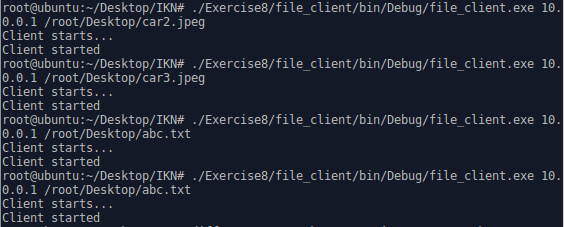
\includegraphics[width=160mm]{figures/Clientstart.png}
			\caption{Eksempler på clientkommandoer}
		\end{figure}

		\begin{figure}[H]
			\centering
			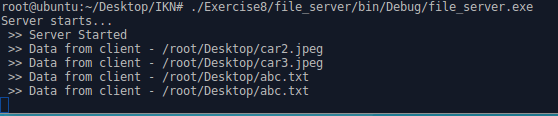
\includegraphics[width=160mm]{figures/Serverstart.png}
			\caption{Eksempler på serversvar på de pågældende clientkommandoer}
		\end{figure}
		
		\begin{figure}[H]
			\centering
			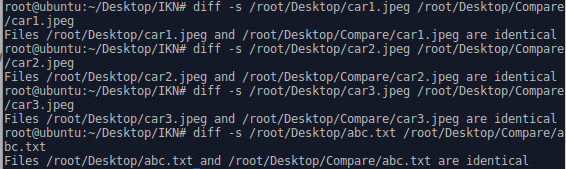
\includegraphics[width=160mm]{figures/compare.png}
			\caption{Test af filernes lighed}
		\end{figure}

\noindent Som det kan ses på ovenstående figurer kører serveren iterativt. Efter serveren er blevet startet bliver den ved med at køre og lytte efter clients. Clients kan så kalde applikationen med parameterene <ip-adresse> <filnavn>, hvorefter serveren sender denne fil til clienten hvis den findes. Ellers reutneres en fejlbesked. Efter filen er blevet modtaget lukker clienten forbindelsen, og en ny client kan komme til.